\documentclass[UTF8,a4paper,12pt]{ctexart}
\usepackage[left=3cm, right=3cm]{geometry}
\usepackage[fontset=mac]{ctex}

\usepackage{amsmath}
\numberwithin{equation}{section}
\renewcommand\thesection{\arabic{section}}
\allowdisplaybreaks[4]       %多行公式中换页
\usepackage{array}
\usepackage[font=small,labelsep=none]{caption}
\usepackage{amssymb}
\usepackage{tikz}
\usepackage{amsthm}
\usepackage{mathrsfs}
\usepackage{float}

\usepackage{dutchcal}
\usepackage{color}
\usepackage{graphicx}    %插入图片 
\usepackage{times}
\usepackage{mathptmx}
\usepackage{fancyhdr} %页眉页脚
\usepackage{booktabs}  %三线表


\pagestyle{fancy}
\fancyhf{}
\fancyfoot[C]{\thepage}

\newcommand*{\circled}[1]{\lower.7ex\hbox{\tikz\draw (0pt, 0pt)%
    circle (.5em) node {\makebox[1em][c]{\small #1}};}}
    
\usepackage{hyperref}  %目录
\hypersetup{colorlinks=true,linkcolor=black}

\renewcommand {\thefigure} {\thesection{}.\arabic{figure}}%设定图片的编号。这样设置的实现效果为图1.1
\renewcommand {\thetable} {\thesection{}.\arabic{table}}


\usepackage{caption}
\captionsetup{font={small},labelsep=quad}%文字5号,之间空一个汉字符位。

\usepackage{appendix}
\usepackage{tocloft} 
\usepackage{titletoc}

\usepackage{setspace}
\usepackage{titlesec}
\setstretch{1.25}


% 设置section字体为黑体三号
\titleformat{\section}{\heiti\zihao{3}\centering}{\thesection}{0.5em}{}[]
% 设置subsection字体为黑体小三号
\titleformat{\subsection}{\heiti\zihao{-3}}{\thesubsection}{0.5em}{}[]
% 设置subsubsection字体为黑体四号
\titleformat{\subsubsection}{\heiti\zihao{4}}{\thesubsubsection}{0.5em}{}[]
%\titlespacing{\section}{0pt}{\baselineskip}{\baselineskip}
%\titlespacing{\section}{0pt}{0pt}{\baselineskip}

% 目录中section的格式
\titlecontents{section}[0pt]{\addvspace{0pt}\filright\heiti\zihao{4}}%
               {\contentspush{\thecontentslabel \quad}}%
               {}{\titlerule*[8pt]{.}\contentspage}
% 目录中subsection的格式
\titlecontents{subsection}[1em]{\addvspace{0pt}\filright\heiti\zihao{5}}%
               {\contentspush{\thecontentslabel \quad}}%
               {}{\titlerule*[8pt]{.}\contentspage}
% 目录中subsubsection的格式
\titlecontents{subsubsection}[2em]{\addvspace{0pt}\filright\songti\zihao{5}}%
               {\contentspush{\thecontentslabel \quad}}%
               {}{\titlerule*[8pt]{.}\contentspage}

\renewcommand{\cftsecleader}{\cftdotfill{\cftdotsep}} %为目录中section补上引导点
               
\makeatletter % 单线页眉
\def\headrule{{\if@fancyplain\let\headrulewidth\plainheadrulewidth\fi%
\hrule\@height 0.5pt \@width\headwidth\vskip1.5pt% 上面线为0.5pt粗
\vskip-2\headrulewidth\vskip-1pt}}     % 与下面正文之间的垂直间距
\makeatother



\setlength{\headheight}{14.48167pt} 
\setlength{\voffset}{-1.14cm}
\setlength{\topmargin}{0cm}
\setlength{\headsep}{2.5cm}


\begin{document}

\thispagestyle{empty}




\begin{center}
\heiti  \zihao{-2} 重庆大学本科学生毕业论文(设计)
\end{center}
%该页为中文扉页。无需页眉页脚,纸质论文应装订在右侧
~\\
\begin{center}
\heiti  \zihao{2} 面向多编程语言的代码检索系统设计与实现
\end{center}
%中文论文标题,1行或2行,黑体,二号,居中。论文题目不得超过36个汉字

~\\
\renewcommand{\headrulewidth}{1pt}
\begin{figure}[htb] 
  \centering
    \center{\includegraphics[width=5cm]  {fig1.png}} 
     \end{figure}
     
~\\
\begin{center}
\heiti\zihao{4}
\begin{tabular}{l}
学\qquad 生:夏劲\\
学\qquad 号:20214966\\
指导教师:刘超\\
专\qquad 业:软件工程\\
\end{tabular}
\end{center}

%此模版适用于理工农医等专业;人文社科类专业按《重庆大学普通本科毕业论文(设计)撰写规范化要求》。  若没有助理指导教师,请删除“助理指导教师姓名”栏。若为校外完成毕业论文(设计),请改为“校外指导教师姓名”即可。  学院、专业填全称。

~\\
\begin{center}
\heiti \zihao{-2} {重庆大学大数据与软件学院}\\
\end{center}

\begin{center}
\heiti \zihao{3} {2025年6月}
\end{center}



\newpage
\thispagestyle{empty}
\setmainfont{Times New Roman}
\begin{center}
\zihao{3}
\textbf{
Undergraduate Thesis (Design) of Chongqing University}
\end{center}
~\\
\begin{center}
\zihao{2}
\textbf{Design and Implementation of a Multi-Programming Language Code Retrieval System}
\end{center}

~\\
\renewcommand{\headrulewidth}{1pt}
\begin{figure}[htb] 
  \centering
    \center{\includegraphics[width=5cm]  {fig1.png}} 
     \end{figure}
     

\setmainfont{Times New Roman}
\begin{center}
\zihao{3} 
\textbf{By}  \\
\textbf{XIAJin}
\end{center}

\begin{center}
\zihao{3} 
\textbf{Supervised by}\\
\textbf{Prof. LIU CHAO}\\
\end{center}

\begin{center}
\zihao{-2} 
\textbf{Software Engineering}\\ %专业
\textbf{	School of Big Data and Software Engineering}\\ %学院
\textbf{Chongqing University}
\end{center}

\begin{center}
\zihao{3} 
\textbf{June,2025}
\end{center}


\newpage
\pagestyle{fancy}
\pagenumbering{Roman}

% 设置左侧页眉
\fancyhead[LH]{ \songti\zihao{-5} 重庆大学本科学生毕业论文(设计)}
\fancyhead[RH]{\songti\zihao{-5} 摘要}



\addcontentsline{toc}{section}{摘要}

\section*{摘\quad 要}
%摘要:二字间空两格,黑体三号居中,段前,段后各空一行。

随着编程语言的多样化和开源项目的迅速增长,开发者在寻找特定代码片段时面临着越来越大的挑战。现有的代码托管平台主要依赖关键词匹配和特定搜索条件进行检索,效率较低且使用门槛较高。大语言模型逐渐成为科研和工业界的热点,利用大语言模型可以轻松将用户的自然语言转译为具有查询功能的条件,并结合具体信息拓展补充用户的查询条件,从而实现更高效的查询体验。本项目旨在利用大语言模型实现一款面向多编程语言的代码检索系统。\par
本文首先介绍了大语言模型的发展情况,并论证了使用大语言模型进行查询条件重写的可行性,强调了提示词工程在这一过程中的重要性。接着简述了前端框架Vue、Visual Studio Code平台的插件开发、Elasticsearch和FastAPI等后台开发框架。根据系统的应用目标,本文进行了系统需求分析,设计了系统架构、功能和数据库结构。在此基础上,本项目开发了基于FastAPI的后台管理逻辑服务、基于Elasticsearch的代码检索服务以及基于DeepSeek-R1的查询重写服务。通过Visual Studio Code平台提供的接口,结合Vue框架实现了Visual Studio Code插件的前端开发,完成了快捷键绑定、项目搜索等一系列功能。\par
本项目开发的面向多编程语言的代码检索系统具有界面美观、操作友好、查询效率高、查询准确等诸多优点。基于FastAPI开发的后台管理系统易于管理和维护,帮助开发人员实现高效的多编程语言项目代码搜索。\par
~\\
\hspace*{2em}{\heiti \zihao{-4}关键词}:代码搜索;Elasticsearch;大模型提示工程\\
%关键字:宋体12磅,行距20磅,段前段后0磅,关键字之间用分号隔开,关键词三个字加粗。

\newpage
\fancyhead[LH]{ \songti\zihao{-5} 重庆大学本科学生毕业论文(设计)}
\fancyhead[RH]{\zihao{-5} ABSTRACT}

\addcontentsline{toc}{section}{ABSTRACT}
\titleformat{\section}[block]{\centering\bfseries\fontspec{Times New Roman}\fontsize{16pt}{20pt}\selectfont}{\thesection}{1em}{}[]

\section*{ABSTRACT}
%ABSTRCT:Times New Roman 加粗三号,段前段后空一行
As programming languages diversify and open-source projects rapidly grow, developers face increasing challenges in finding specific code snippets. Existing code hosting platforms primarily rely on keyword matching and specific search conditions, resulting in low efficiency and a high usage threshold. Large language models have become a hot topic in both research and industry. By leveraging these models, users' natural language can be easily translated into functional query conditions, which can be further expanded with specific information to enhance the query experience. This project aims to implement a code retrieval system for multiple programming languages using large language models.\par

This paper first introduces the development of large language models and demonstrates the feasibility of using them for query condition rewriting, highlighting the importance of prompt engineering in this process. It then briefly describes the front-end framework Vue, plugin development for the Visual Studio Code platform, and back-end development frameworks such as Elasticsearch and FastAPI. Based on the system's application goals, a system requirements analysis was conducted, and the system architecture, functionality, and database structure were designed. On this basis, the project developed a back-end management logic service based on FastAPI, a code retrieval service using Elasticsearch, and a query rewriting service using DeepSeek-R1. The front-end development of the Visual Studio Code plugin was achieved through the platform's provided interfaces, combined with the Vue framework, implementing features such as shortcut key bindings and project search.\par

The code retrieval system developed in this project for multiple programming languages offers numerous advantages, including an aesthetically pleasing interface, user-friendly operation, high query efficiency, and accuracy. The back-end management system developed with FastAPI is easy to manage and maintain, aiding developers in efficiently searching for code across multi-language projects.\par 
%英文摘要内容:Times New Roman 12磅(即小四号),行距20磅段前段后0磅

~\\ 
\hspace*{2em}\textbf{Key words}: Code Search;Elasticsearch;LLM Prompt\\
%Keywords:Times New Roman 12磅,行距20磅, “key words” 两词加粗

\newpage
\fancyhead[LH]{ \songti\zihao{-5} 重庆大学本科学生毕业论文(设计)}
\fancyhead[RH]{\songti\zihao{-5} 目录}

\renewcommand\contentsname{{目\quad 录}}

\begin{center}
{\tableofcontents
\thispagestyle{fancy}
\fancyhead [RO, L] {\zihao{-5}{\songti 1\quad 绪论}}
\fancyhead [LO, R] {\zihao{-5}{\songti 重庆大学本科学生毕业论文(设计)}}
}
\end{center}



\newpage
\fancyhead[LH]{\zihao{-5}{\songti 重庆大学本科学生毕业论文(设计)}}
\fancyhead[RH]{\zihao{-5}{\songti 1\quad 绪论}}
\pagenumbering{arabic}


\titleformat{\section}{\heiti\zihao{3}\centering}{\thesection}{0.5em}{}[]
\section{绪论}
\subsection{研究目的及意义}
\zihao{-4} 
随着机器学习、深度学习等人工智能技术的快速发展,这些高新技术在解决传统领域挑战中发挥了重要作用。在搜索领域,传统搜索服务提供商通常直接采用Elasticsearch作为搜索引擎来完成信息检索。然而,传统搜索引擎基于倒排索引的检索方式要求用户提供极其精确的搜索词,并掌握一定的搜索技巧,这极大地限制了普通用户的搜索体验。随着人工智能技术,尤其是大语言模型(LLM)的进步,利用其自然语言友好特性来辅助搜索已成为科研界和工业界的研究热点。\par
Elasticsearch是一种分布式、RESTful风格的搜索和分析引擎,其强大的搜索能力源于其独特的倒排索引结构(Inverted Index)。这种数据结构使Elasticsearch具备高效的全文搜索能力、实时数据处理能力以及高可扩展性,同时能够处理结构化和非结构化数据。\par
大型语言模型(LLM)是拥有海量参数和卓越学习能力的高级语言模型,其核心模块是Transformer架构中的自注意力机制。自注意力机制作为语言建模任务的基本构建块,能够有效处理顺序数据,实现并行化计算,并捕捉文本中的远程依赖关系。LLM的显著优势在于其能够理解自然语言并执行基于自然语言的指令,这对用户侧软件服务非常友好。然而,LLM的另一特点是其庞大的模型参数和极高的训练成本。从头预训练一个大型模型所需的资源(如数百万高性能显卡卡时)是普通实验室或个人工作者难以承担的。因此,针对特定场景的任务,工业界普遍采用开源的大语言模型进行监督微调(SFT),或通过Prompt工程来实现任务目标。\par
本项目旨在构建一个面向多编程语言的代码检索系统,该系统将融合大语言模型的自然语言友好能力,实现对用户搜索词的重写、完善,结合Elasticsearch强大的多结构文本搜索能力实现用户方便快速搜索多语言项目的能力。同时我还讲相关能力集成到Visual Studio Code平台,发布免费的开源插件,为所有开发者提供便捷高效的代码搜索服务。


\subsection{国内外研究现状}
\zihao{-4} 
2004年,Shay Banon创造了Elasticsearch的前身——Compass。在Compass的基础上,Shay Banon进一步实现了分布式和可扩展性优化,并提供了HTTP接口,使得Java以外的语言也能调用。2010年,Elasticsearch的第一个版本正式发布。\par
Elasticsearch是一种成熟的搜索解决方案,一些大型搜索公司如Google和百度都基于Elasticsearch进行研发。Elasticsearch支持RESTful风格的调用,客户端可以通过HTTP请求直接操作Elasticsearch服务。它还提供了多种客户端支持,包括Java、Python、Go、PHP等语言的SDK,以及JDBC、ODBC等标准化接口。Elasticsearch广泛应用于全文搜索、日志分析、实时数据分析、地理空间搜索以及商业智能领域的数据聚合分析。在部署方面,Elasticsearch支持单节点模式,适用于开发和测试环境,可以通过简单的Docker命令快速启动。在生产环境中,通常采用分布式集群部署,通过分片(Shard)和副本(Replica)机制实现水平扩展和高可用性。集群节点可以动态扩容并自动平衡数据负载,同时支持主节点、数据节点、协调节点等角色划分,以优化资源分配。\par
在大语言模型方面,基于Transformer架构的大语言模型如OpenAI的GPT系列、Google的Gemini、Meta的Llama、腾讯的混元系列模型等,都已经在自然语言处理领域展现出强大的能力。这些模型通过海量数据训练,能够理解和生成高质量的自然语言文本。在Transformer基础上,大语言模型继续发展,得益于多专家(MoE)架构、多模态融合以及自监督学习等技术创新,其在代码语义理解、跨语言检索等场景中的潜力被进一步释放。例如,GitHub Copilot基于GPT系列开发的Codex模型,能够完成代码补全和跨语言语义关联;Google推出的Gemini Code Assist则通过多专家架构优化了代码检索的响应速度和准确性。与此同时,模型自我反思机制成为提升代码生成可靠性的关键技术突破,以DeepSeek R1为代表的反思模型通过强化学习框架实现自我校验与动态优化,其采用的图谱重标定(GRPO)算法可对代码逻辑进行多步验证,在Math-500测试中达到97.3\%的准确率,并在Codeforces编程竞赛中超越96\%的人类选手。该模型通过冷启动训练策略融合监督微调与自我对弈机制,不仅能在代码生成过程中主动识别变量定义错误、逻辑矛盾等问题,还能通过语言反馈链重构搜索词表达,显著提升多编程语言检索的语义对齐度。当前主流模型如Llama 3和通义千问已通过指令微调集成类似反思机制,使得代码检索系统的查询意图理解误差率较传统模型降低42\%。\par

\subsection{论文研究内容}
\zihao{-4} 
本项目以构建一款面向多编程语言的化代码检索系统为目标,基于Elasticsearch构建分布式搜索引擎内核,集成LLM(Large Language Model)实现搜索意图理解与查询词重构,通过FastAPI搭建高性能异步后端服务,并采用Vue3响应式框架开发可视化交互界面,最终以Visual Studio Code插件形态实现IDE深度集成,为开发者提供语义级代码检索能力\par
整个系统架构分为四大核心模块:\par
第一部分,​代码采集与预处理:基于Scrapy框架构建分布式爬虫,通过GitHub API获取主流编程语言的开源代码,采用AST解析技术实现代码片段结构化提取,并完成开源协议合规性校验。\par
第二部分,​存储与索引构建:部署Elasticsearch集群,设计BM25算法与稠密向量混合索引结构,集成IK分词插件优化专业术语处理,支持代码语法特征与语义特征的双重表征。\par
第三部分,​检索服务实现:基于Gin框架开发RESTful API接口,采用异步IO机制提升高并发性能,设计融合关键词匹配、向量相似度计算及上下文权重的混合搜索算法,实现毫秒级响应。\par
第四部分,​交互界面开发:使用Vue3 Composition API构建渐进式前端应用,通过VSCode Extension API实现IDE插件集成,支持代码快捷搜索、交互式代码预览等功能。\par

\subsection{论文组织架构}
\zihao{-4} 
第一章,绪论。阐述了本研究的目的和背景,并分析当前国内外的搜索技术和大模型研究现状,概述了本论文的主要研究内容。\par
第二章,相关理论和技术。通过对大模型与提示工程相关技术的介绍,阐明了本研究选择大模型作为搜索词重写基石的原因,并介绍开发多编程语言代码检索系统所使用的技术框架。\par
第三章,系统需求分析与设计。对系统进行需求分析后,以此设计流程完整的应用程序。\par
第四章,系统后端应用层实现。\par
第五章,系统前端表现层实现。\par


\newpage
\fancyhead[LH]{\zihao{-5}{\songti 重庆大学本科学生毕业论文(设计)}}
\fancyhead[RH]{\zihao{-5}{\songti 2\quad 正文文字格式}}

\section{相关理论和技术}
\subsection{大语言模型}
\zihao{-4} 
大语言模型是实现本系统搜索功能的核心技术。要深入理解当前的大语言模型,必须先了解其核心架构——Transformer。因此,本节将简要介绍Transformer及大语言模型的其他关键技术。
\subsubsection{Transformer}
Vaswani等人指出,循环神经网络模型(RNN)在每个时间步都需要依赖前一时间步的隐藏状态信息进行计算,这种固有的顺序依赖性使得RNN难以在多GPU上进行并行计算,从而限制了RNN在处理超大规模文本数据时的训练能力。为了解决这一问题,他们提出了Transformer架构,这是一种完全依赖注意力机制连接编码器和解码器的网络架构。Transformer显著提高了训练的并行度和速度。后续的一系列研究表明,基于Transformer架构的预训练模型(pre-trained models / pre-trained language models,PTM / PLM)在各种任务上都能实现最先进的性能表现,因此,Transformer已成为自然语言处理(NLP)领域的首选架构。除了在语言相关领域的应用之外,Transformer还被广泛应用于计算机视觉、音频处理以及自然科学学科,如化学、生物等领域。\par
\begin{figure}[H] 
	\center{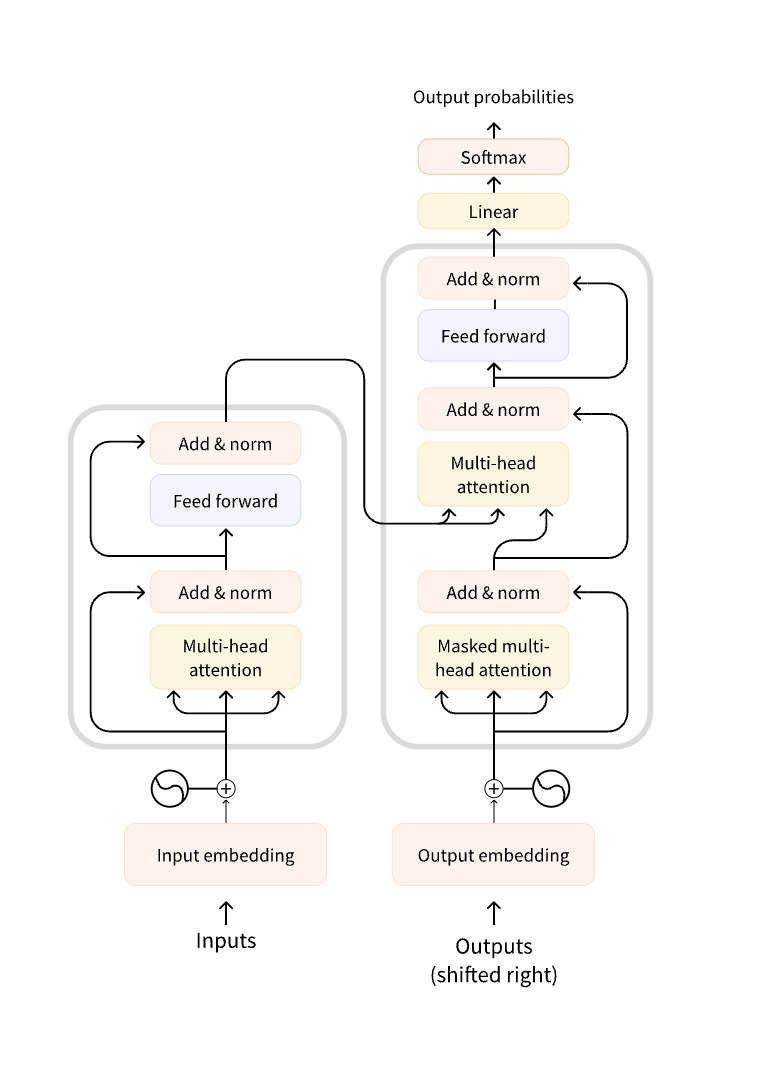
\includegraphics[width=0.95\textwidth]  {transformer.png}} 
	\caption{Transformer结构}
	\label{transformer}
\end{figure} %图表上下各空一行
Transformer架构如图\ref{transformer}所示,其整体由编码器(图\ref{transformer}左)和解码器(图\ref{transformer}右)组成。每个编码器块由多头注意力机制模块和位置前馈网络组成,模块间使用残差连接,并配有层归一化模块;解码器块在位置前馈网络和多头自注意力模块之间插入了交叉注意力模块,其中的自注意力模块用于组织某个位置信息对后续位置信息的影响。下面将简要介绍上述几种重要模块:\par
(1) 多头注意力机制:让序列中的每一个元素学习并计算与其他元素的互注意力分数权重,如公式\ref{func_1}所示:
\begin{eqnarray}
	\text{Attention(Q,K,V)} =  \text{softmax}(\frac{QK^T}{\sqrt[]{d_k}})V
	\label{func_1}
\end{eqnarray}
但Transformer并不只是简单应用了单个注意力函数,而是使用了多头注意力机制将 \(d_m\) 维度的原始 \(Q\)、\(K\)、\(V\) 分别线性投影到 \(d_k\)、\(d_k\)、\(d_v\) 维度,再根据公式\ref{func_1}进行注意力计算,整体公式如下:
\begin{eqnarray}
	\mathrm{MultiHead(Q,K,V)=~Concat(head_{1},...,head_{h})W^{O}} \\
	\mathrm{where~head_{i}~=~Attention(QW_{i}^{Q},KW_{i}^{K},VW_{i}^{V})}
	\label{func_2}
\end{eqnarray}
Transformer利用多头注意力机制能够同时关注到来自不同位置的且具有不同表示的子空间信息,增强了架构的表达能力。\par
(2) 位置前馈网络:全连接前馈网络模块,用于接收自注意力模块的输出:\par
\begin{eqnarray}
\mathrm{FFN}(x) & =\max(0,x\mathrm{W}_1+\mathrm{b}_1)\mathrm{W}_2+\mathrm{b}_2 \\
& =\mathrm{~ReLU(H'W}_1+\mathrm{b}_1)\mathrm{W}_2+\mathrm{b}_2
\label{func_3}
\end{eqnarray}
(3) 残差连接与归一化:Transformer 在每个模块间使用残差连接,然后进行层归一化。其中编码器块表示为:\par
\begin{eqnarray}
	\mathrm{H^{\prime}=~LayerNorm(Self~Attention(X)+(X)} \\
	\mathrm{H=~LayerNorm(FFN(H^{\prime})+(H^{\prime})}
	\label{func_4}
\end{eqnarray}
\subsubsection{混合专家模型}
\begin{figure}[H]
	\center{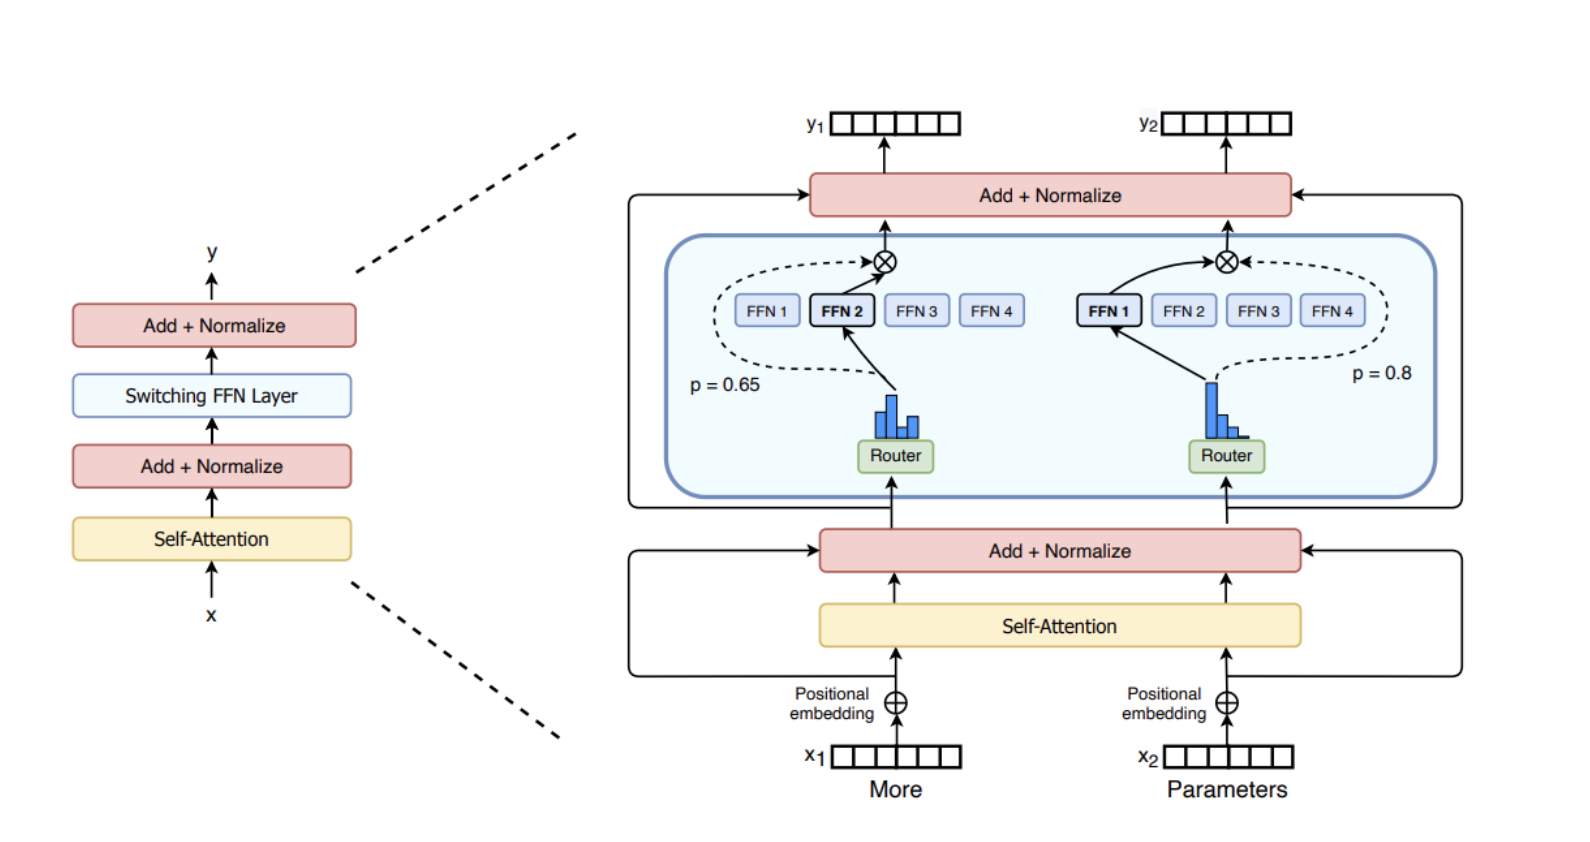
\includegraphics[width=0.95\textwidth]  {MoE.png}} 
	\caption{MoE结构}
	\label{MoE}
\end{figure}
Google Brain团队发现传统Transformer架构在扩展到超大规模时面临计算资源消耗激增的问题,尤其是前馈网络层(FFN)的全参数激活机制导致训练和推理效率急剧下降。为此,他们提出基于混合专家模型(Mixture of Experts, MoE)的稀疏架构改造方案,通过将Transformer中的FFN层替换为动态路由的专家网络集合,实现计算效率与模型容量的平衡。MoE架构如图\ref{MoE}所示,其核心创新在于引入稀疏门控机制(图\ref{MoE}蓝色部分),该机制由可学习的路由网络构成,针对每个输入词元生成专家选择概率分布,仅激活概率最高的前K个专家(通常K=2-4),其余专家保持非激活状态。具体而言,每个MoE层包含N个独立的前馈网络作为专家(例如N=8或32),其数学表达为:
\begin{eqnarray}
	\mathrm{MoE}(x)=\sum_{i=1}^KG(x)_i\cdot E_i(x)
	\label{func_5}
\end{eqnarray}
其中$G(x)$为门控网络输出的Top-K权重,$E_i(x)$为被选中的专家网络输出。这种设计使得模型总参数量可扩展至万亿级别,而实际计算量仅与激活专家数相关。实验表明,Switch Transformer在同等计算资源下,训练速度较传统稠密模型提升4倍,且推理时内存占用降低至1/4。进一步地,通过引入噪声注入(Noisy Top-K Gating)和负载均衡损失函数,MoE有效缓解了专家利用率不均衡问题,例如GLaM模型以1.2万亿参数仅激活97亿参数即达到GPT-3的97\%性能。当前,MoE架构已在GPT-4、DeepSeek、Mixtral 8x7B等主流大模型中广泛应用,成为突破单一模型规模瓶颈的核心技术路径。
\subsubsection{提示词工程}
提示(Prompt)是一系列提供给LLM的指令,我们可以通过自定义提示来增强、改善LLM的能力。Reynolds等人首次系统性地提出Prompt作为调控大型语言模型(LLM)行为的核心接口,其本质是通过自然语言指令或结构化模板显式定义输入规范、处理规则及输出约束,从而动态重构LLM的上下文推理路径以适配特定任务需求。比如,可以指定LLM在生成文档时标记重点内容;可以指定LLM只输出符合要求的关键词语;可以指定LLM只生成指定代码风格的代码等。\par
提示工程(Prompt Engineering)作为一种独特的编程模式,主要围绕向大型语言模型(LLM)精准输入提示展开操作。本质上,这一过程需要精心设计适配的提示模板,以此助力完成特定的下游任务。实践表明,优化提示内容能够显著提升模型在各类任务中的表现。\par
\begin{figure}[H]
	\center{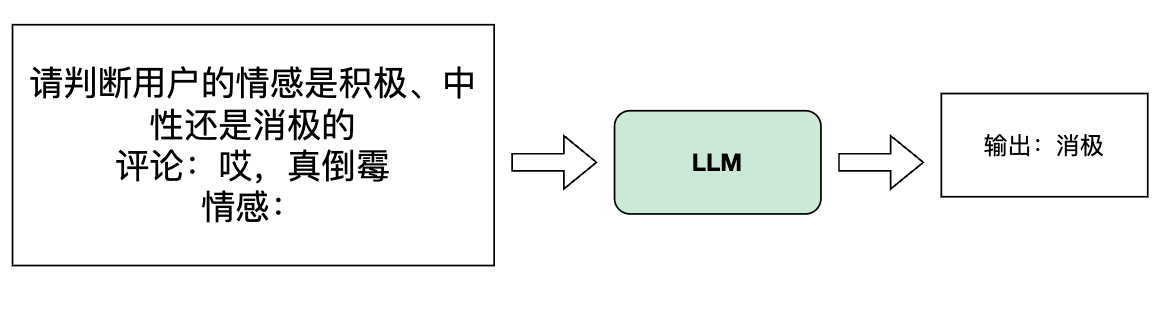
\includegraphics[width=0.95\textwidth]  {zero_shot.png}} 
	\caption{零样本提示示例}
	\label{zero_shot}
\end{figure}
\begin{figure}[H]
	\center{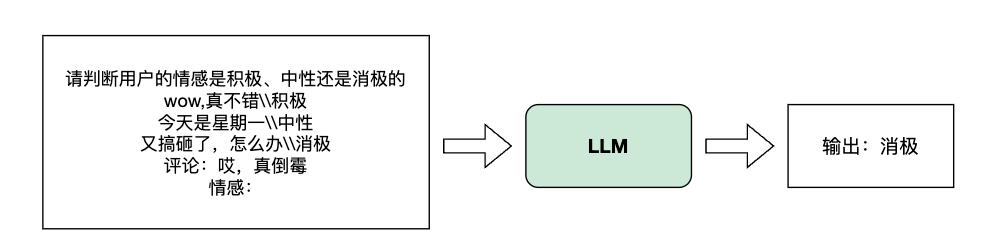
\includegraphics[width=0.95\textwidth]  {few_shot.png}} 
	\caption{少样本提示示例}
	\label{few_shot}
\end{figure}
在提示工程的实际应用中,零样本提示(Zero-Shots Prompting)是一种基础方法,图\ref{zero_shot}展示了相关示例。该方法下,即便不向模型提供任何参考示例,模型也能够给出有价值的回应,完成既定任务。然而,当零样本提示无法满足需求时,少样本提示(Few-Shots Prompting)便派上用场,如图\ref{few_shot}。此时,需针对下游任务设计专门的提示模板,模板不仅要囊括一系列LLM处理规则,还要为后续待输入文本预留特定位置。在向LLM发起询问时,只需将待输入文本填充至提示模板预留空位,即可构建完整提示。除此之外,开启思维链、给LLM指定角色性格等提示技巧都能显著改变LLM输出效果和对任务的执行情况。\par
进一步看,巧妙构建提示能够催生全新的交互模式。例如,借助提示指令,LLM可生成与软件工程概念相关的测验题目,模拟程序运行流程,甚至模拟命令行终端窗口的交互场景。不仅如此,提示还具备自适应特性,部分提示能够依据当前情况,推荐其他提示,以便收集更多信息,或生成相关成果物。提示的这些进阶功能,充分彰显了深入设计提示、挖掘其在简单文本与代码生成之外价值的重要意义。 
\subsection{Elasticsearch}
\zihao{-4} 
Elasticsearch 是一个开源的分布式搜索和分析引擎,它被设计用来快速地存储、搜索和分析海量数据,在面向多编程语言的代码检索系统中发挥着重要的作用。面对各种类型的复杂数据,传统的数据库系统在处理搜索和分析任务时往往显得力不从心,而Elasticsearch凭借其强大的功能和优异的性能脱颖而出。它提供了 RESTful API,高效的全文搜索能力,多语言支持,分布式架构和实时搜索特性,使得系统能够快速、准确地检索到数百万个开源项目文件中的相关代码,提供了便捷的代码检索服务。
\subsubsection{Elasticsearch 的核心概念}
索引(Index):在Elasticsearch中,索引是具有相似特征的文档集合,类似于关系型数据库中的数据库。在面向多编程语言的代码检索系统里,一个索引可以对应一种编程语言的所有开源项目文件,或者是所有语言的综合代码文件集合。在项目中,创建了一个名为code的索引,用于存储所有语言的开源代码文件。值得注意的是在Elasticsearch中索引是一个逻辑空间的概念,这和分片(shard)的概念相互区分。\par
分片(Shard)和副本(Replica):为了实现分布式存储和提高系统的可用性与性能,Elasticsearch 引入了分片和副本的概念。分片是将一个大的索引拆分成多个较小的部分,每个分片可以独立存储在不同的节点上,这样可以并行处理搜索请求,提高搜索效率。副本是分片的复制,每个分片可以有多个副本,当某个节点出现故障时,副本可以接替其工作,保证系统的正常运行。在代码检索系统中,对于数百万个开源项目文件的索引,
可以通过合理设置分片和副本的数量,来优化系统的性能和可靠性。\par
\begin{figure}[H]
	\center{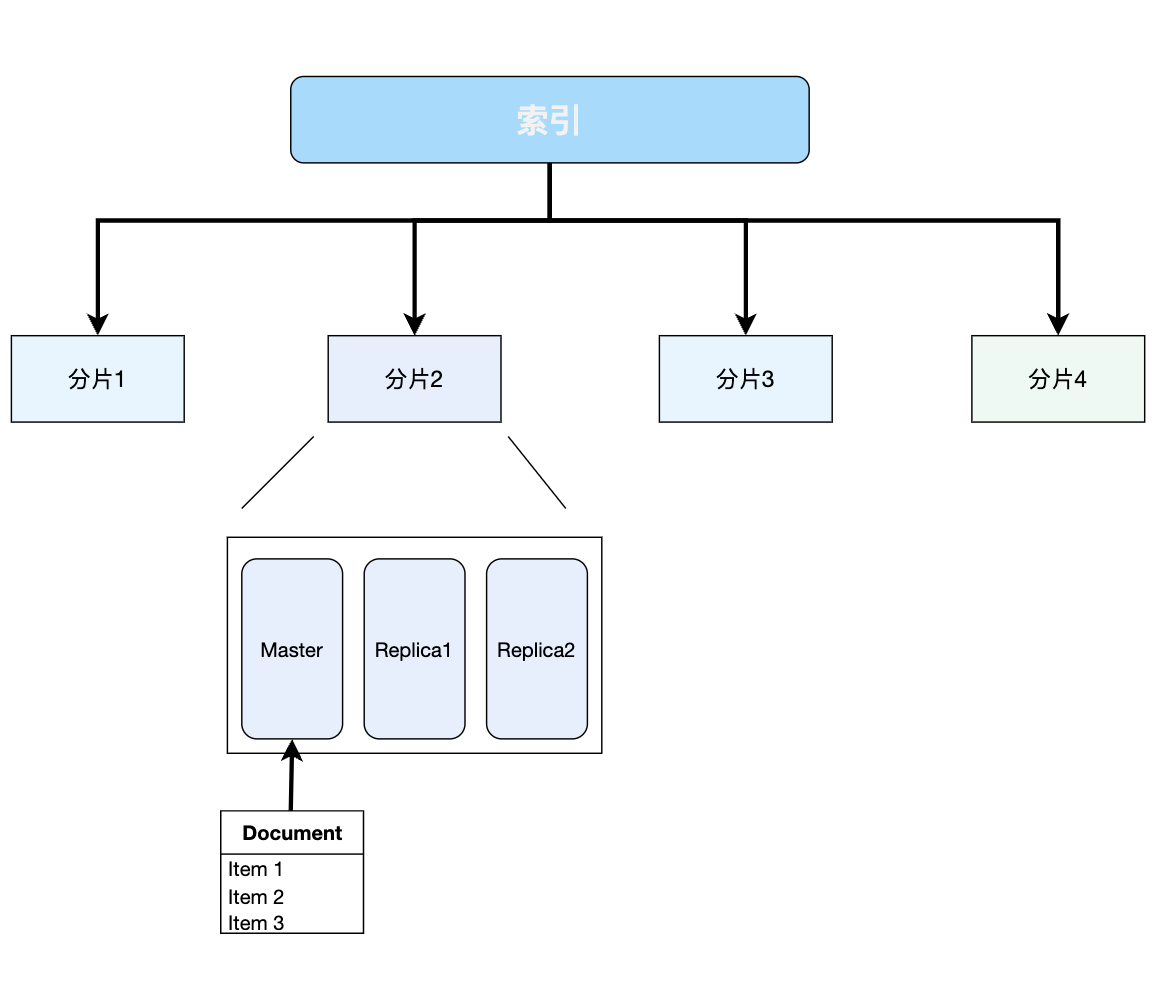
\includegraphics[width=0.95\textwidth]  {Elasticsearch.png}} 
	\caption{Elasticsearch结构}
	\label{Elasticsearch}
\end{figure}
文档(Document):文档是Elasticsearch中可被索引的最小数据单元,它以JSON格式表示,类似于关系型数据库中的行。在代码检索系统里,一个文档可以对应一个具体的代码文件,包含文件名、代码内容、开源协议、星数等信息。\par
\subsection{Visual Studio Code插件}
\zihao{-4}
为了高效构建美观且用户友好的交互界面,Visual Studio Code通过支持TypeScript或JavaScript实现其官方接口,显著简化了开发流程。此外,VS Code允许在侧边栏(Side Bar)中嵌入WebView页面,这一特性为开发者提供了利用前端框架开发插件的可行性,极大降低了技术学习门槛。在持续开发与维护前端项目时,选择成熟框架已成为关键策略。Vue.js作为主流前端框架,已迭代至Vue 3版本。其庞大的开源生态(如Element Plus等UI组件库)为开发者提供了丰富的可视化资源,即使缺乏专业设计支持,也能快速构建出美观的界面。相较于前代版本,Vue 3在响应式系统、组件化开发及性能优化等方面引入了多项革新性改进。本章节将系统性地介绍Vue.js框架的核心特性,\par
\subsubsection{Vue框架}
Vue.js是一套渐进式JavaScript框架,凭借其轻量级架构、低学习门槛、高效性能等核心优势,已成为全球范围内最受欢迎的前端框架之一。作为渐进式框架的典型代表,Vue.js的设计以灵活性为核心原则,开发者可根据实际需求逐步采用其提供的功能模块,而非强制要求一次性全面使用所有特性。这种渐进式特性使其既能满足小型项目的快速开发需求,又能支撑大型应用的复杂架构。\par
在设计模式方面,Vue采用模型-视图-视图模型(Model-View-ViewModel,MVVM)架构(图\ref{MVVM}所示)。相较于传统的MVC模式,Vue的MVVM模式实现了视图与模型的解耦,并通过视图模型(ViewModel)层实现数据的无缝双向绑定。该模式通过数据绑定和视图自动更新机制,显著减少了冗余代码的编写,使开发者能够将精力集中于核心业务逻辑与界面设计的优化。\par
\begin{figure}[H]
	\center{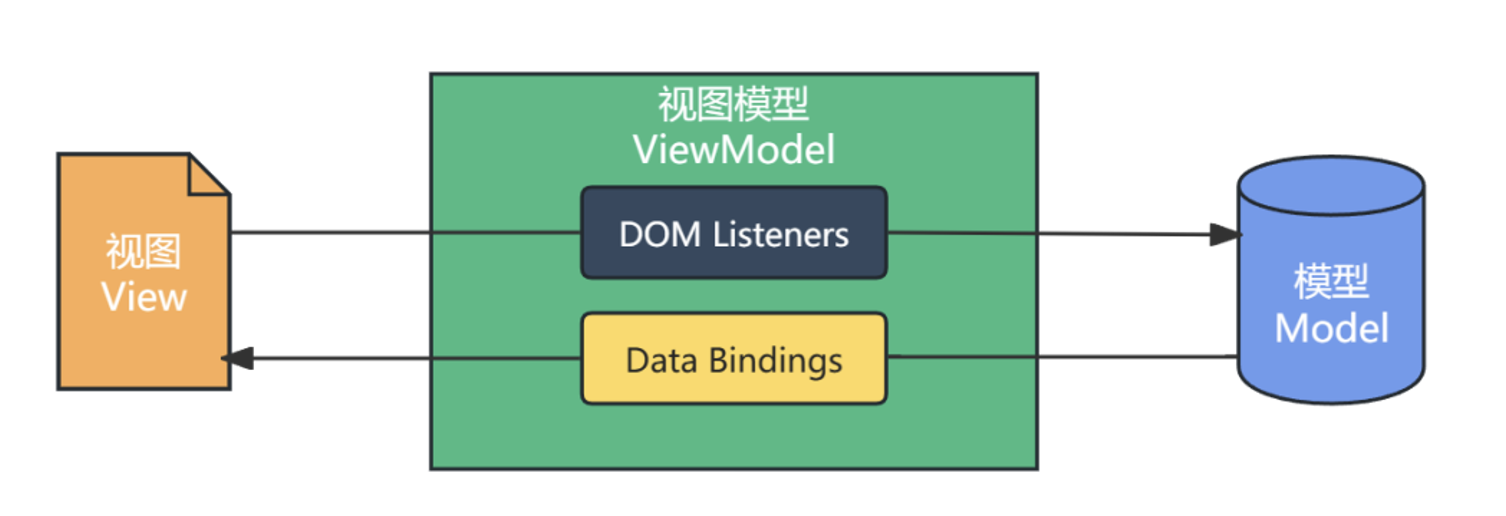
\includegraphics[width=0.95\textwidth]  {MVVM.png}} 
	\caption{Vue的MVVM设计模式}
	\label{MVVM}
\end{figure}
在技术特性方面,Vue.js引入了虚拟DOM(Virtual DOM)与响应式数据系统。其中,响应式系统通过实时追踪状态变化,能在数据更新时智能驱动视图的局部渲染,从而大幅减少直接操作DOM的频率。这一机制不仅降低了开发复杂度,更避免了频繁调用DOM对象的性能损耗,使开发者得以专注于业务逻辑的实现。\par
\subsection{本章小结}
\zihao{-4} 
本章介绍了实现面向多编程语言的代码检索系统的核心理论和技术。首先探讨了大语言模型及其核心架构Transformer。Transformer通过多头注意力机制、位置前馈网络、残差连接与归一化等模块,解决了传统循环神经网络在并行计算和处理超大规模文本数据时的局限性,成为自然语言处理领域的首选架构。此外,混合专家模型(MoE)通过稀疏门控机制有效提升了模型的计算效率和容量,成为突破单一模型规模瓶颈的重要技术路径。另外强调了通过精心设计提示模板来增强和改善大语言模型能力的重要性。提示工程不仅能够提升模型在各类任务中的表现,还能催生全新的交互模式,充分挖掘大语言模型在文本与代码生成之外的潜力。随后探讨了Elasticsearch在多编程语言代码检索系统中的应用。Elasticsearch作为一个开源的分布式搜索和分析引擎,凭借其高效的全文搜索能力和分布式架构,能够快速、准确地检索海量数据,提供便捷的代码检索服务。最后,介绍了Visual Studio Code插件的开发,特别是Vue.js框架的应用。Vue.js以其轻量级架构和渐进式特性,结合虚拟DOM和响应式数据系统,为开发者提供了高效的前端开发体验。通过这些技术的结合,本系统能够实现高效、准确的代码搜索和用户友好的交互界面。

\newpage
\fancyhead[LH]{\zihao{-5}{\songti 重庆大学本科学生毕业论文(设计)}}
\fancyhead[RH]{\zihao{-5}{\songti 3\quad 系统需求分析与设计}}

\section{系统需求分析与设计}
本章主要介绍面向多编程语言的代码检索系统的系统需求分析与设计工作,包括系统需求分析、系统架构设计、业务功能设计和数据库设计。首先从用户需求和系统的功能性与非功能性需求出发,对面向多编程语言的代码检索系统进行深入的需求分析。接着,根据需求分析的结果,对系统进行详细的解析,设计总体架构和前后端服务架构。然后,进行系统的业务功能设计,重点设计项目存储、大模型提示词工程等关键功能模块。
\subsection{系统需求分析}
\zihao{-4} 
\subsubsection{用户需求}
本系统的核心目标是为开发人员提供高效便捷的代码检索支持,通过智能化的自然语言搜索能力辅助开发流程,显著提升代码复用效率与开发质量。特别针对涉密场景需求,系统支持完全离线化部署方案,可在无网络环境下实现对本地化代码仓库的检索功能。系统主要面向两类核心用户群体:开发人员与系统运维人员。整体用户需求示意图如图\ref{flow}所示。
\begin{figure}[H]
	\center{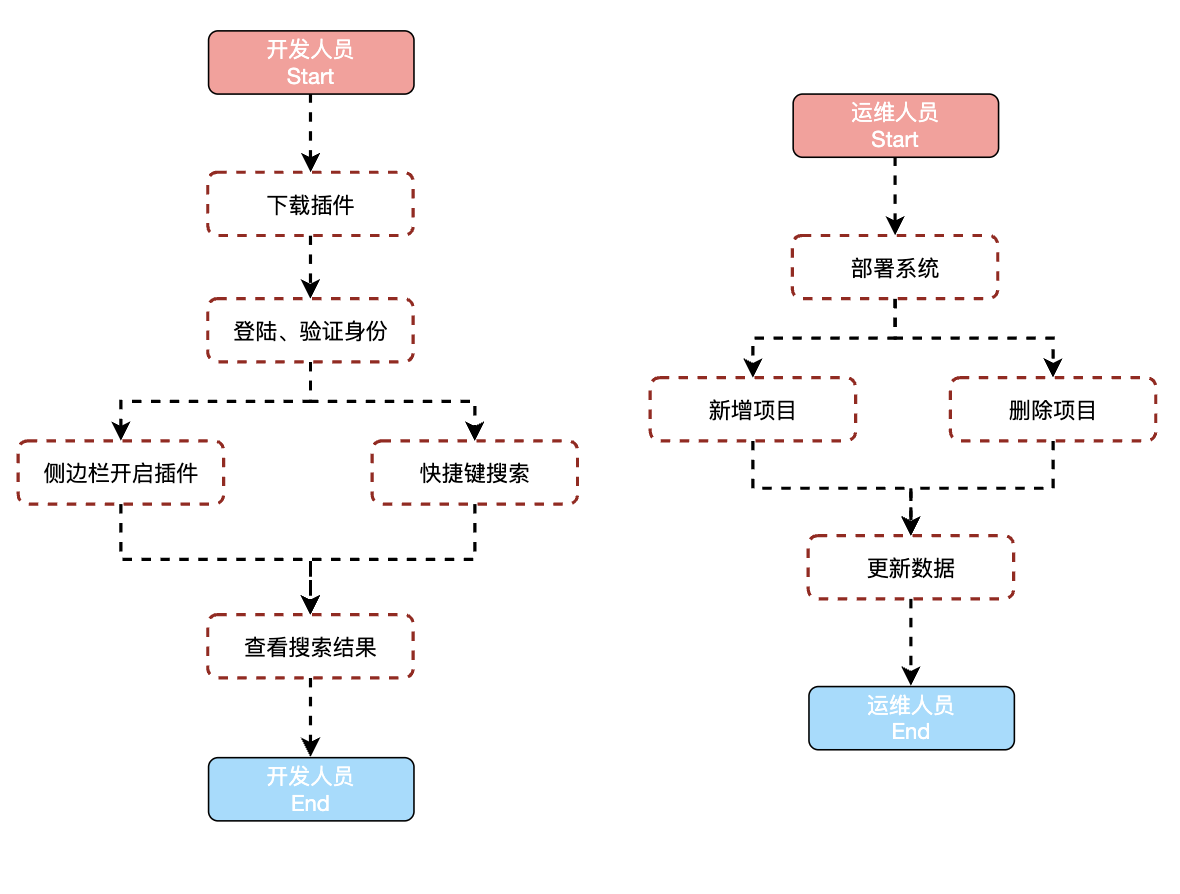
\includegraphics[width=0.95\textwidth]  {flow.png}} 
	\caption{整体用户需求示意图用例图}
	\label{flow}
\end{figure}
\subsubsection{系统功能性需求分析}
本节将根据用户需求,明确系统核心功能性需求,本小节根据系统不同角色定位,做如下功能性需求分析:\par
对于开发者用户,做如下功能分析,图\ref{user}为开发人员的功能需求用例图:\par
\begin{figure}[H]
	\center{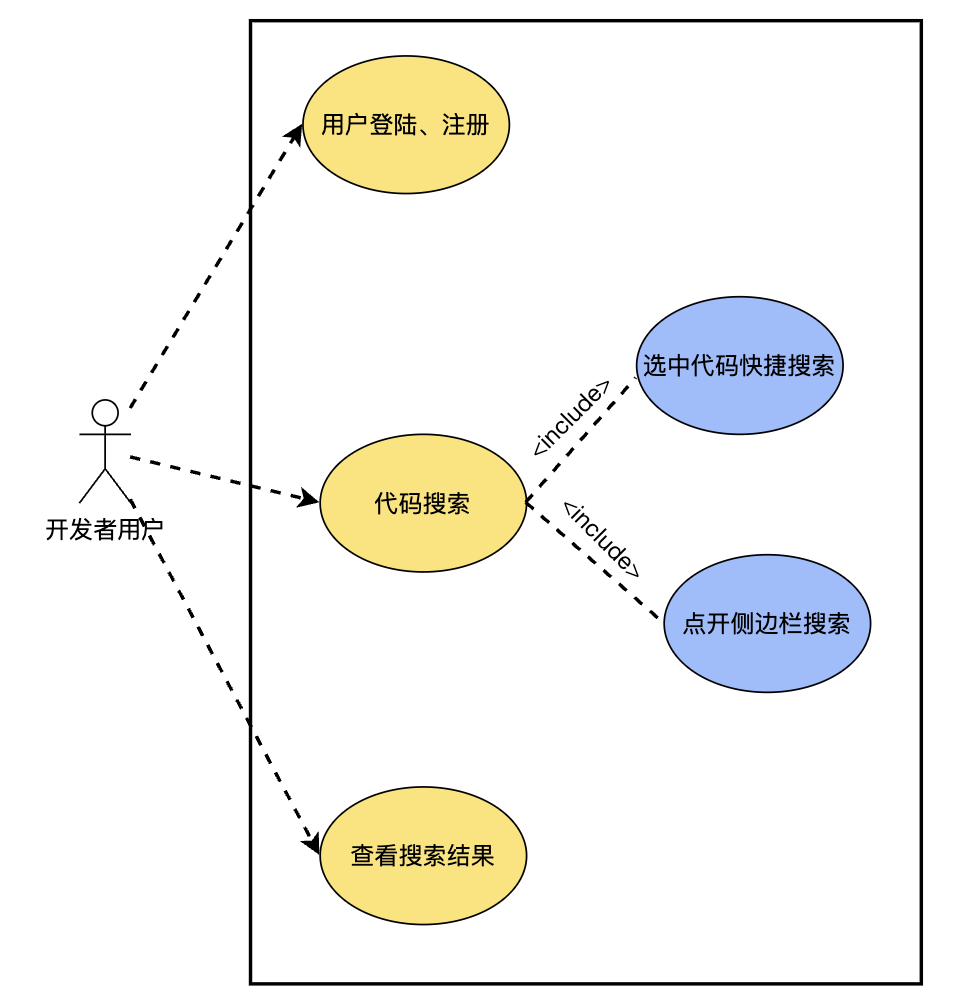
\includegraphics[width=0.95\textwidth]  {user_use.png}} 
	\caption{开发者用户用例图}
	\label{user}
\end{figure}
(1)开发者用户注册:开发者用户下载系统后,由系统弹窗提示用户在未登录状态,此时用户可以选择登陆或者注册。如果用户选择注册,则跳转注册页面,用户输入邮箱号后,通过验证码自动完成注册。\par
(2)开发者用户登陆:开发者用户下载系统后,由系统弹窗提示用户在未登录状态,此时用户可以选择登陆或者注册。如果用户选择登陆,则跳转登陆页面,用户输入绑定邮箱后,经过验证,成功完成登陆。\par
(3)代码搜索:开发者用户在使用VS Code编码过程中,可以通过绑定的快捷键,直接跳转搜索界面。如果此时鼠标选中了代码,则自动将代码复制到用户的系统粘贴面板上;用户也可以点击侧边的插件icon,跳转到搜索界面,手动输入搜索关键词开始搜搜。\par
(4)查看搜索结果,用户在搜索完成后,如果有搜索结果,可点击搜索结果框,通过链接自动跳转项目详情。\par
对于运维人员,做如下功能分析,图\ref{operator}为运维人员的功能需求用例图:\par
\begin{figure}[H]
	\center{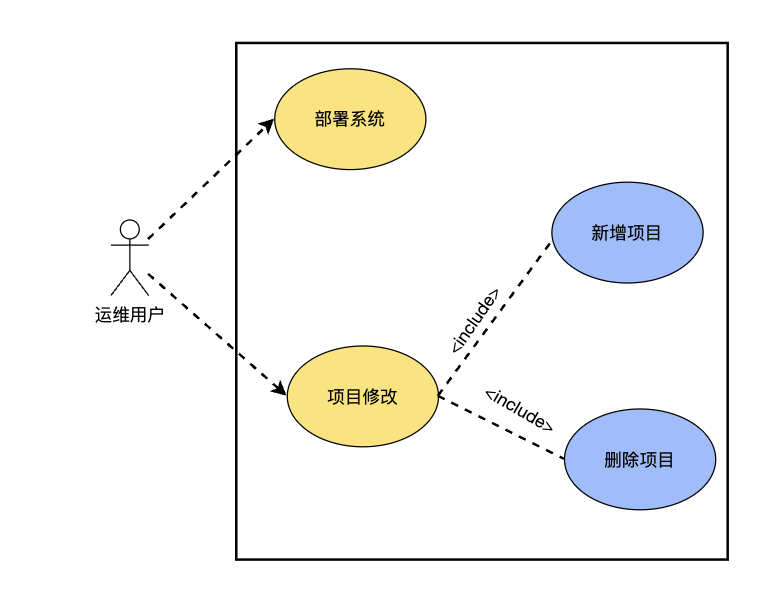
\includegraphics[width=0.95\textwidth]  {operator_user.png}} 
	\caption{运维用户用例图}
	\label{operator}
\end{figure}
(1)系统部署:运维人员能根据系统提供的指示,安装系统必要的依赖,完成系统的部署、迁移。\par
(2)项目修改:运维人员能根据项目变动,灵活新增或者删除Elasticsearch中管理的项目。\par
\subsubsection{系统非功能性需求分析}
(1)	易用性:本系统在界面布局上应当符合使用者的实际习惯与需求,应具备逻辑性和直观性,用户在进行操作时应该能够清晰地了解每个功能的用途和位置,操作流程和反馈信息也应该及时、明确。界面应该呈现出清晰、统一的信息组织结构,将不同功能和信息分类展示,让用户能够快速获取到有用的项目信息\par
(2)	拓展性:本系统应该满足可拓展需求。在前端表现层,能够快速拓展对后续需求页面,对已使用组件做到有效复用。在后端应用层,能够满足后端需求灵活变更,对新增需求和更变需求,通过利用已有功能模板快速开发。\par
(3)	可靠性:本系统的可靠性需求,主要体现在用户登录、项目搜素,大模型改写方面。具体来说,系统需要保障可靠的用户登录体验;实现可靠的搜索体验;大语言模型在改写用户提示词的时候应该确保不随意篡改用户的本意,达到提升搜索准确性等效果。\par
(4)	安全性:本系统在安全性上,做到用户间严格分离,不可跨越权限操作。需要设计具备数据备份、恢复功能的数据库处理方法,保障数据库信息安全。\par
\subsection{系统架构设计}
\subsubsection{系统总体架构设计}
面向多编程语言的代码检索系统整体将采用前后端分离的方式进行组织。可以分为前端交互层、后端逻辑层以及数据层三个维度,如图\ref{all_structure}所示。前端交互层使用Vue框架编写交互逻辑,使用ElementUI渲染前端图形化页面和可视化模块。后端使用Gin框架编写应用服务,规范API风格,接受前端请求,同时负责和数据层和大语言模型进行交互,实现主要的搜索逻辑。数据层使用Elasticsearch管理所有的项目数据。
\begin{figure}[H]
	\center{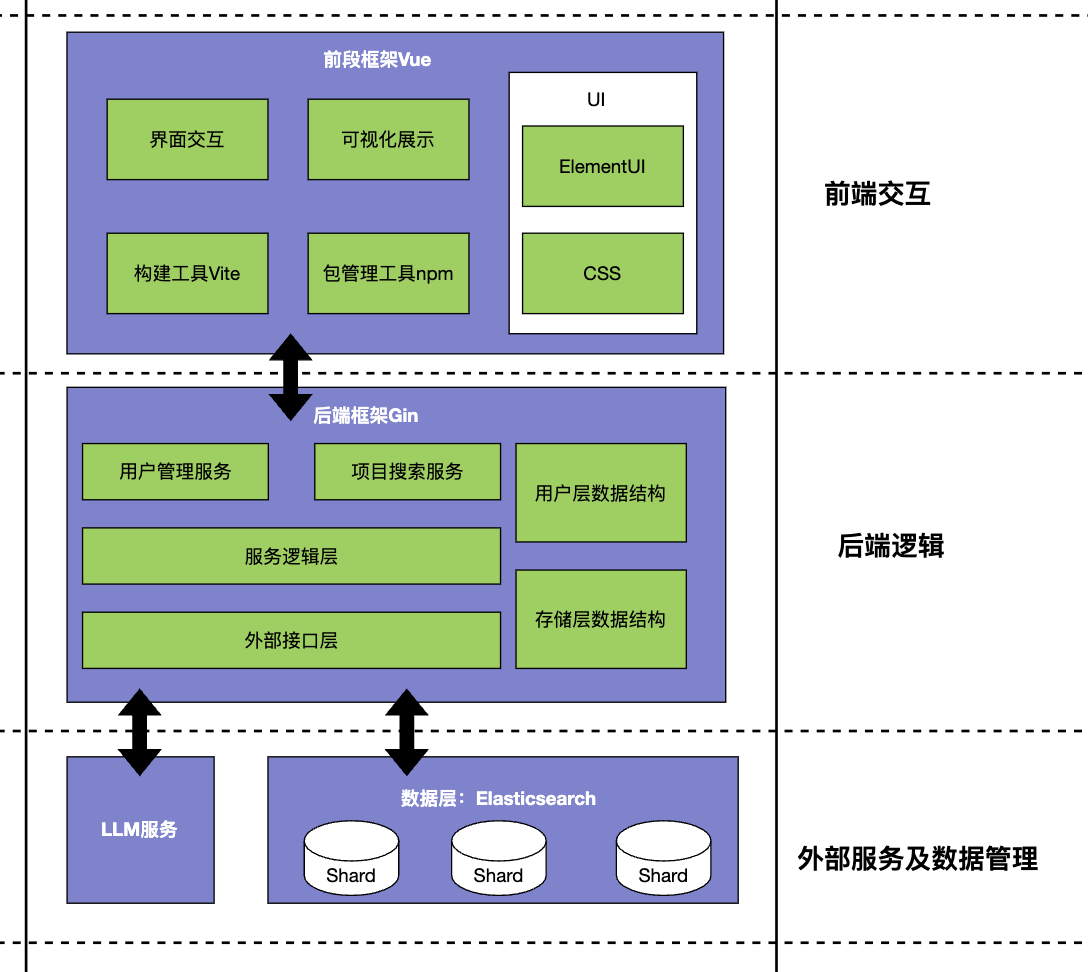
\includegraphics[width=0.95\textwidth]  {structure.png}} 
	\caption{系统总体架构图}
	\label{all_structure}
\end{figure}
\begin{table}[htbp]
\centering
\caption{高频感应加热的基本参数}
\small
\begin{tabular}{c c c c}
\toprule
感应频率 &感应发生器功率 & 工件移动速度  &感应圈与零件间隙\\
(KHz)&($\% \times$80Kw) &(mm/min)  &(mm)\\
\midrule
250 &88 &5900 &1.65\\

250 &88 &5900 &1.65\\

250 &88 &5900 &1.65\\

250 &88 &5900 &1.65\\



\bottomrule
\end{tabular}
\end{table}



\begin{table}[htbp]
\centering
\captionsetup{singlelinecheck=off}
\caption*{续表3.1}
\small
\begin{tabular}{c c c c}
\toprule
感应频率 &感应发生器功率 & 工件移动速度  &感应圈与零件间隙\\
(KHz)&($\% \times$80Kw) &(mm/min)  &(mm)\\
\midrule
250 &88 &5900 &1.65\\

250 &88 &5900 &1.65\\
\bottomrule
\end{tabular}
\end{table}
\vspace{\baselineskip}
%表格太大需要转页时,需要在续表上方注明“续表”,表头也应重复排出。


\subsection{公式格式}


\begin{eqnarray}
\frac{1}{\mu} \nabla^2A - j \omega \sigma A -\nabla(\frac{1}{\mu}) \times(\nabla \times A)+J_0=0
\end{eqnarray}


\subsection{本章小结}
\zihao{-4} 
本章介绍了……

\newpage
\fancyhead[LH]{\zihao{-5}{\songti 重庆大学本科学生毕业论文(设计)}}
\fancyhead[RH]{\zihao{-5}{\songti 4\quad 结论与展望}}
\section{结论与展望}

\subsection{主要结论}
\zihao{-4} 
本文主要……

\subsection{研究展望}
\zihao{-4} 
更深入的研究……

\newpage
\fancyhead[LH]{\zihao{-5}{\songti 重庆大学本科学生毕业论文(设计)}}
\fancyhead[RH]{\zihao{-5}{\songti 参考文献}}

\addcontentsline{toc}{section}{参考文献}
\renewcommand\refname{参考文献}

\zihao{5}

\begin{thebibliography}{1}
\setlength{\itemsep}{0pt}
\bibitem{1} 杨瑞林, 李力军. 新型低合金高强韧性耐磨钢的研究[J]. 钢铁. 1999(7): 41-45.
\bibitem{2} 于潇, 刘义, 柴跃廷, 等. 互联网药品可信交易环境中主体资质审核备案模式[J]. 清华大学学报(自然科学版), 2012, 52(11): 1518-1523.
\bibitem{3} Schinstock D.E., Cuttino J.F. Real time kinematic solutions of a non-contacting, three dimensional metrology frame[J]. Precision Engineering. 2000, 24(1): 70-76. 
\bibitem{4} 温诗铸. 摩擦学原理[M]. 北京: 清华大学出版社, 1990: 296-300.
\bibitem{5} 蒋有绪, 郭泉水, 马娟, 等. 中国森林群落分类及其群落学特征[M]. 北京: 科学出版社, 1998: 5-17.
\bibitem{6} 贾名字. 工程硕士论文撰写规范[D]. 重庆: 重庆大学, 2000: 177-178.
\bibitem{7} 张凯军. 轨道火车及高速轨道火车紧急安全制动辅助装置: 201220158825.2[P]. 2012-04-05.
\bibitem{8} 全国信息与文献标准化技术委员会. 文献著录: 第4部分 非书资料: GB/T 3792.4-2009[S]. 北京: 中国标准出版社, 2010: 3.
\end{thebibliography}
%(参考文献格式请参考GB/T 7714-2015《信息与文献 参考文献著录规则》)

\newpage
\fancyhead[LH]{\zihao{-5}{\songti 重庆大学本科学生毕业论文(设计)}}
\fancyhead[RH]{\zihao{-5}{\songti 附录A:XX公式的推导}}

\addcontentsline{toc}{section}{附录A:XX公式的推导}
\section*{附录A:XX公式的推导}
\zihao{5}
XX公式的推导过程是:

\newpage
\fancyhead[LH]{\zihao{-5}{\songti 重庆大学本科学生毕业论文(设计)}}
\fancyhead[RH]{\zihao{-5}{\songti 致谢}}

\addcontentsline{toc}{section}{致谢}
\section*{致\quad 谢}
\zihao{-4}
致谢主要感谢导师和对论文工作有直接贡献和帮助的人士和单位。致谢言语应谦虚诚恳,实事求是。

\newpage
\thispagestyle{empty}

\addcontentsline{toc}{section}{原创性声明和使用授权书}
\begin{center}
\heiti \zihao{3}
原创性声明
\end{center}

\songti\zihao{-4}
郑重声明:所呈交的论文(设计)\underline{《  \hspace{6em}》},是本人在导师的指导下,独立进行研究取得的成果。除论文(设计)中已经标注引用的内容外,本论文(设计)不包含其他人或集体已经发表或撰写过的作品成果。对本文的研究做出贡献的个人和集体,均已在文中以明确方式标明。本人完全意识到本声明的法律后果,并承诺因本声明而产生的法律结果由本人承担。

~\\
\begin{flushleft}
\begin{tabular}{l}
\songti\zihao{-4}
论文(设计)作者签名: \underline{\hspace{6em}}\\
\songti\zihao{-4}
日期:\underline{\hspace{6em}}
\end{tabular}
\end{flushleft}

~\\
\begin{center}
\heiti \zihao{3}
使用授权书
\end{center}

\songti\zihao{-4}
本论文(设计)作者完全了解学校有关保留、使用论文(设计)的规定,同意学校保留并向国家有关部门或机构送交论文(设计)复印件和电子版,允许论文(设计)被查阅和借阅。本人授权重庆大学将本论文(设计)的全部或部分内容编入有关数据库进行检索,可以采用影印、缩印或扫描等复制方式保存和汇编本论文(设计)。

~\\
\songti\zihao{-4}
本论文(设计)属于:\par
保\quad 密 $\Box$  \quad 在\underline{\qquad}年解密后适用本授权书\par
不保密 $\Box$

~\\
~\\
\begin{flushleft}
\songti\zihao{-4}
\begin{tabular}{l l}
论文(设计)作者签名:\underline{\hspace{6em}} \hspace{300mm}&指导教师签名:\underline{\hspace{6em}} \\
日期:\underline{\hspace{6em}} &日期:\underline{\hspace{6em}}\\
\end{tabular}
\end{flushleft}

\end{document} 